\chapter{Languages}
\label{chap:languages}
\graphicspath{{chapters/languages/}}


\lstdefinestyle{customcode}{
	frame=single,
	numbers=right,
	numbers=left,
	xleftmargin=2em,
	framexleftmargin=1.8em,
	numberstyle=\color{gray},
}

This chapter contains description and examples of several languages and programming environment used to implement parallel and distributed applications.

\section{Message Passing Library}

\section{Task Based Programming Models}
\subsection{PaRSEC}
PaRSEC \cite{BBDHL2011} \cite{BBDFH2013} (Parallel Runtime Scheduling and Execution Controller) is an engine for scheduling tasks on distributed hybrid environments.

It offers a flexible API to develop domain specific languages.
It aims to shift the focus of developers from repetitive architectural details toward meaningful algorithmic improvements.
Two domain specific languages are supported by Parsec, the Parameterized Task Graph \cite{DBBHD2014} (PTG) and Dynamic Task Discovery \cite{HoHBD2017} (DTD)

In PTG \cite{DBBHD2014}, users would use a parameterized expression of task dependencies combined with PaRSEC which would implicitly infer the communication between nodes and the accelerators.
The users has to provide a description of the data flow of their application and the tasks which are applied on the data.
They also has to provide the tasks that are the source of the data and the tasks that are the destination.
So, this is a compressed algebraic representation of the task graph.
Then, it is transformed into C code using a pre-compiler.
Users need to understand and provide all the data flow of their algorithm to use this model.


DTD \cite{HoHBD2017} is a task-based programming paradigm which provides an alternative way to express task dependency in PaRSEC that achieves a similar purpose to PTG.
Contrary to PTG where users had to express tasks in a parameterized manner, DTD allows them to write sequential constructs (ifs, loops, etc\dots) to insert tasks in PaRSEC.
The tasks are given to the runtime with the data they will use and their mode of usage.
Then, the runtime will compute dependencies out of data pointers used by the tasks.
In a distributed system, the data movements among the nodes are completely implicit.


\begin{figure*}
\lstinputlisting[style=customcode,language=C,
caption=Task in PaRSEC\label{lst:parsec_task}]{chapters/languages/parsec_task.c}
\end{figure*}


\subsubsection{Task definition}
Listing \ref{lst:parsec_task} shows how to define a task in PaRSEC.
Line 1 defines the name of the task and the integer parameters in input.
This task is called \textit{PMM}.
Line 3 and 4 give the range of those parameters.
In line 6, \textit{dcA} is a data descriptor and is used to align the task on the resources from the descriptor.
Line 8 to 11 describe the dependencies of the task.
Line 13 to 19 are the body of the task.
They contain the computations on the data.
This task calls the \textit{pmm\_core} to process the data stored in the \textit{Ap} and \textit{Bp} pointers.


\subsubsection{Dependency definition}
Line 8 to 11 from Listing \ref{lst:parsec_task} shows how to describe the dependencies of a task in PaRSEC.
The \textit{PMM} task uses two pieces of data \textit{A} and \textit{Inv}.
They are temporary pointers that hold the data that will be used in the task.

\textit{A} is in read-write mode (RW).
It means \textit{PMM} expects a pointer in input that will be called A in the body of the task.
That pointer can be modified and will be transfered into another task.
The data in \textit{A} come from the part $(i,k)$ in the data descriptor \textit{dcA} when $k=0$ and from the data referenced as \textit{$A_{ij}$} in the task \textit{PMM\_D}.
When the task is finished, the data in \textit{A} will be sent as input of \textit{$A_{ik}$} from the task \textit{PMM\_D}.
Indeed, Listing \ref{lst:parsec_pmmd_dep} shows the corresponding dependencies definition.
We find \textit{A} from \textit{PMM} as input for \textit{$A_{ik}$} from \textit{PMM\_D} and \textit{$A_{ij}$} as input for \textit{A} from \textit{PMM}.

\textit{Inv} is in read mode (READ).
It only uses the piece of data named \textit{Inv} from the \textit{Inv} task.

There is also a write mode (WRITE) that output a new piece of data.

Control dependencies can also be added through the \textit{CTL} keyword.
It allows the user to create control flow data which can tell the runtime if a task has to be done before another one.

\begin{figure*}[h]
\lstinputlisting[style=customcode,language=C,
caption=Expression of PMM\_D dependencies\label{lst:parsec_pmmd_dep}]{chapters/languages/parsec_pmmd_dep.c}
\end{figure*}

This way of expressing the dependencies is error-prone.
Indeed, the user can easily be lost in the definition of the dependencies since he has to replicate them in two tasks (for instance, the input of a task is the output from another one).
Moreover, it can become very complicated when there is a lot of different tasks and condition on the parameters.

\subsubsection{Data definition}
\textit{dcA} is a \textit{two\_dim\_block\_cyclic\_t*}.
This is a matrix data type provided by PaRSEC.
It helps to store two dimensional arrays of matrices in memory.
We use it to store sub-matrices in our block-based LU factorization.
It extends the initial data type \textit{parsec\_ddesc\_t} as for each data type used by PaRSEC.
Listing \ref{lst:parsec_custom_datatype} shows how to extend \textit{parsec\_ddesc\_t} to create a data type called \textit{my\_datatype\_t}.

This data distribution descriptor stores only one data block per MPI process in the field \textit{ptr}, of size \textit{size} bytes.
However, the user's memory is not manipulated directly by PaRSEC.
It uses \textit{parsec\_data\_t*} as well as \textit{parsec\_data\_copy\_t*}.
\textit{parsec\_data\_t} is an abstract representation of user data.
\textit{parsec\_ddesc\_t} class instantiates at most one per MPI process per user data element.
\textit{parsec\_data\_copy\_t} is a representation of a copy of the user data and multiple instances can exist at the same time.
Distributed Data Descriptors usually manipulate parsec\_data\_t objects, and provide parsec\_data\_copy\_t objects, using PaRSEC functions to instantiate them.


\begin{figure*}[h]
\lstinputlisting[style=customcode,language=C,
caption=PaRSEC custom datatype definition\label{lst:parsec_custom_datatype}]{chapters/languages/parsec_custom_datatype.c}
\end{figure*}

PaRSEC uses all fields from the \textit{parsec\_ddesc\_t} object.
The user has to fill them in order to implement a new data type.
\textit{myrank} is the rank of the local MPI process.
\textit{nodes} is the number of nodes in the MPI Communicator.
Then, the other obligatory fields are function pointers.
\textit{rank\_of} and \textit{rank\_of\_key} return the rank of a given data element, based on its multidimensional index or its flat key.
\textit{vpid\_of} and \textit{vpid\_of\_key} return the identifier of the Virtual Process that "owns" a data identified by its multidimensional index or its flat key.
\textit{data\_of} and \textit{data\_of\_key} return the parsec\_data\_t* associated with the user data at this multidimensional index position, or for this flat key.

Line 3 to 9 in Listing \ref{lst:parsec_launch} shows how to initialize \textit{dcA} with a built-in function dedicated to that and then how to allocated the memory in each MPI process with \textit{parsec\_data\_allocate} function.

With the definition of these functions, PaRSEC is able to manage efficiently the data from the user.


\subsubsection{Graph execution}
PaRSEC compiler generates code to launch the tasks.
In this case, it is the \textit{parsec\_lu\_new} function as shown in Listing \ref{lst:parsec_launch}.
It takes \textit{dcA} the data descriptor and \textit{bm} which is the number of tiles in each dimension as parameter.
The preprocessor finds them in the source file and put them as input parameters of the function to launch the tasks.

\begin{figure*}
\lstinputlisting[style=customcode,language=C,
caption=PaRSEC tasks launching\label{lst:parsec_launch}]{chapters/languages/parsec_launch.c}
\end{figure*}


\subsubsection{Granularity}
PaRSEC assigns computation threads to the cores, overlaps communications and computations.
Each task is run into a thread.
Furthermore, PaRSEC tasks are fine grain.

\subsubsection{Tasks re-usability}
Tasks cannot be reused as they are since their dependencies, parameter ranges and alignment are stored in the task definition.
They have to be rewritten for each new application.
However, core computations can be stored into a routine which can be reused into other tasks.

\subsubsection{Scheduling}
The design of the PARSEC runtime system focuses on scalability.
PaRSEC tries to limit task knowledge to processes that are responsible for their execution.
The scheduling decisions are entirely distributed.
Algorithmic correctness should not require control synchronization, and synchronous collective synchronization should be avoided.


\subsubsection{Type of graph}
PaRSEC is mainly based on the expression of data flow dependencies but the user can also give additional control flow dependencies if needed.

\subsubsection{GPU support}
In PTG, the tasks are implemented for CPU by default.
However, PaRSEC is able to move data to the GPU and to call tasks on it.
The code to run on GPU is specified in the \textit{BODY} as for a CPU task and adding the option \textit{[type=CUDA]} to
after the keyword \textit{BODY}.
A function which operates on the data on the GPU can be called in the body of the task.


\subsection{Legion}
Legion \cite{BaTSA2012} is a data-centric parallel programming model.
It aims to make the programming system aware of the structure of the data in the program.
Legion provides explicit declaration of data properties (organization, partitioning, privileges, and coherence) and their implementation via the logical regions.
They are the fundamental abstraction used to describe data in Legion applications.
Logical regions can be partitioned into sub-regions and data structures can be encoded in logical regions to express locality describing data independence.

A Legion program executes as a tree of tasks spawning sub-tasks recursively.
Each tasks specifies the logical region they will access.
With the understanding of the data and their use, Legion can extract parallelism and find the data movement related to the specified data properties.
Legion also provides a mapping interface to control the mapping of the tasks and the data on the processors during the execution of the application.

Legion installation is a bit different than other libraries.
It is not installed as a compiled library.
The user has to compile it each time he compiles an application.
A static library is generated while executing the Makefile provided to compile an application and is included in the executable.
Therefore, compiling an application is taking some time.

\begin{figure*}
\lstinputlisting[style=customcode,language=C,
caption=Legion task\label{lst:legion_task}]{chapters/languages/legion_task.c}
\end{figure*}

\subsubsection{Task definition}
Legion tasks are implemented as a tree of tasks.
The main function calls Legion runtime to register the top level task which will spawn other tasks.
Those task will also spawn other tasks.
Line 36 from Listing \ref{lst:legion_task} shows how to call Legion runtime to launch the tasks.
Tasks have to be registered into Legion using a \textit{Registrar}.
Line 31 to 34 shows how to do that and bind the task to use CPUs.

Legion tasks need to have generic parameters so that the runtime can call them and pass the data and pieces of information they need.
Line 1 to 3 shows the prototype of a function which is used as a task in Legion.
This task expect two regions which store data that will be accessed in this task and a integer as argument since the task asserts that the size of the region is two (line 4 and 5) and that the length of the arguments is of the size of an integer (line 8).

Data regions are accessed through \textit{FieldId} and \textit{FieldAccessor}.
Line 12 and 15 shows how to get accessors to a region in read mode.
It can be used with an \textit{Iterator} on an index space (as defined on line 18).
This iterator is used as index to the accessors so that pieces of data can be retrieved or set as shown on line 24.


\begin{figure*}[t]
\lstinputlisting[style=customcode,language=C,
caption=Legion data\label{lst:legion_data}]{chapters/languages/legion_data.c}
\end{figure*}

\subsubsection{Dependency definition}
Dependencies are implicitly defined with the access mode of the regions and the tree of tasks.
Indeed, a task can launch another tasks when it is finished.

\subsubsection{Data definition}
Data are defined through regions of any given type.
To define a region and divide it in sub-regions then run tasks on the sub-regions, an index space and a field space for the region have to be defined.
The index space keeps the coordinates of the values in the multi-dimensional array represented by a region (line 8 from Listing \ref{lst:legion_data}).
The field space defines which type of data there will be in the region (line 9 to 15 from Listing \ref{lst:legion_data}).
It is represented by a number of byte for each coordinate of the field space.
Furthermore, they can be combined into a \textit{LogicalRegion}  (line 16 from Listing \ref{lst:legion_data}).
It will allocate the region of the designed type in memory.
Custom mappers can be used to optimize the data allocation.

This \textit{LogicalRegion} is split into two partitions; a regular block partition and a partition with ghost borders (duplicated values between neighbor sub-regions).
It is done by defining another index space which will record the coordinates of the sub-regions (line 19 from Listing \ref{lst:legion_data}).
Then, the index partitions can be created from the data index space and the sub-regions index space (line 21 to 29 from Listing \ref{lst:legion_data}).
Finally, the \textit{LogicalPartition} which contains the split data can be created from the initial \textit{LogicalRegion} and the newly defined sub-regions index partitions (line 31 to 34 from Listing \ref{lst:legion_data}).


\subsubsection{Graph execution}
The tasks are registered into the runtime system then the user can use the runtime to start executing the tasks from the tree of tasks.

\begin{figure*}
\lstinputlisting[style=customcode,language=C,
caption=Legion launch task\label{lst:legion_task_launch}]{chapters/languages/legion_task_launch.c}
\end{figure*}

There is several way of launching tasks in Legion.
Tasks can be launched on a \textit{LogicalRegion} and  the task will process all the data of the region.
They can also be launched on all the sub-regions of a \textit{LogicalPartition} at the same time then the scheduler manage the resources on which launch the tasks.
Listing \ref{lst:legion_task_launch} shows how to process sub-regions in this way.
An \textit{IndexLauncher} need to be created to do so.
It needs the identifier of the task which is defined when registering the task, the sub-regions index space on which launch the tasks and arguments for the tasks.
The \textit{LogicalPartition} have to be given to the index launcher so that the tasks can access the data.
This is performed by using the \textit{add\_region\_requirement} and the \textit{add\_field} methods.
These parameters are passed to the task via the runtime as we saw in Listing \ref{lst:legion_task}.
Then we can tell the runtime to execute the tasks with the \textit{execute\_index\_space} method (Line 13 in Listing \ref{lst:legion_task_launch}).

\subsubsection{Granularity}
Tasks are run as thread by the runtime so tasks are fine-grain.

\subsubsection{Tasks re-usability}
Tasks can be registered and launched in another application if it provides the regions and parameters expected by the task.

\subsubsection{Scheduling}
Legion uses a software out-of-order processor (SOOP) to schedule tasks.
It dynamically schedules a stream of tasks.
It is constrained by region dependences.
It is also pipelined, distributed, and extracts nested parallelism from subtasks.
Legion uses a \textit{deferred execution model} which separates the issuing of the operations from when operations are executed.
An issued operation waits for other operations on which it is dependent to complete before executing without blocking the scheduler.

\subsubsection{Type of graph}
Legion tasks are defined as a tree of tasks.

\subsubsection{GPU support}
Legion supports data migrations to GPUs.
Data are accessed through Legion data structure.
Tasks are implemented in C++ and can be launched on GPU.
The user has to create tasks (a C++ class) that extends a Legion \textit{Launcher} (for instance, \textit{IndexLauncher}) and to implement a \textit{cpu\_base\_impl} function to run the task on CPU and a \textit{gpu\_base\_impl} to run on GPU.
When the user register the task, he has to specify that the task will run on GPU.

\subsection{Regent}
Regent \cite{SLTBA2015} is a programming model which simplifies Legion.
Regent compiler translates Regent programs into efficient implementations for Legion.
It results in programs that are written with fewer lines of codes and at a higher level.

\subsubsection{Task definition}
A Regent task is similar to a function.
It is defined with the \textit{task} keyword until the keyword \textit{end}.
It has parameters after the name of the task (\textit{pmm\_d} in Listing \ref{lst:regent_task}).
Regent tasks also need \textit{coherence modes} to specify how the data will be accessed.
They can be in \textit{reads}, \textit{writes} or both modes.
On line 4 from Listing \ref{lst:regent_task}, there is an example of read access mode for \textit{B} as well as read and write access mode for \textit{A}.
Line 5 to 12 are the computations in the task.


\begin{figure*}
\lstinputlisting[style=customcode,
caption=Regent task\label{lst:regent_task}]{chapters/languages/regent_task.rg}
\end{figure*}

\begin{figure*}
\lstinputlisting[style=customcode,
caption=Regent application\label{lst:regent_main}]{chapters/languages/regent_main.rg}
\end{figure*}

\subsubsection{Dependency definition}
Dependencies between tasks are automatically inferred by Regent compiler from input modes.
Line 35 to 43 from Listing \ref{lst:regent_main} show examples on how to call a task in Regent.
This limits the parallelism that can be detected and create additional dependencies when the system is not sure that the tasks are independent.


\subsubsection{Data definition}
Data types are stored in regions.
The regions can be partitioned and tasks can be executed on subregions.
Custom types can be defined and used as base in regions.
Regions are multi-dimensional arrays.

Line 24 to 27 from Listing \ref{lst:regent_main} define a partitioned region A.
First, the index space of the region itself is created.
Then, the index space of the partition is created.
It is a 2D array of size $nt * nt$ where $nt$ is the number of sub-region in each dimension.
The region \textit{A} can be created out of the index space of the region in line 26.
It creates a 2D region of doubles.
Finally, \textit{A} can be divided in sub-regions.
To do that, the function \textit{make\_partition\_mat} which is defined in line 6 is used.
This function puts each point in \textit{A} into a sub-region.
It is done by using coloration.
Each point is given a color and goes into one of the sub-region.
This function separates the initial region into regular blocks.

The data in an index space are accessed using an \textit{int2d} data structure.
It represents the coordinates of the point.
Each sub-region keeps the index space of the initial region.
Therefore, the lower bound is added to the \textit{int2d} while accessing the values in the task (line 8 in Listing \ref{lst:regent_task}).
\textit{int2d} are also used to access sub-regions as in line 40 of Listing \ref{lst:regent_main}.


\subsubsection{Graph execution}
The tasks are launched through the main function.
Regent compiler converts code into Legion code so the tasks are executed using Legion execution model.
Main function is registered into Regent using \textit{start} function (line 46 from \ref{lst:regent_main}).
It is the starting point of the application.


\subsubsection{Granularity}
Tasks are run as Legion tasks.
They are run into a thread.
Furthermore, they are fine-grain tasks.

\subsubsection{Tasks re-usability}
Tasks can be reused.
They can be stored in another regent file which can be included in another application.
Then, tasks can be called as they are from the other application.

\subsubsection{Scheduling}
Legion scheduling policy is used here.

\subsubsection{Type of graph}
As Regent code is converted in to Legion code, Regent uses Legion tree of tasks that are spawn recursively starting from the main task.

\subsubsection{GPU support}
Regent supports generation of CUDA code for Legion.
A task can be converted to GPU code instead of CPU code by annotating the task with \textit{\_\_demand(\_\_cuda)}.
Regent will then generate CUDA code for Legion that will be executed by Legion runtime.


\subsection{TensorFlow}
TensorFlow \cite{AABBC2016} (\url{https://www.tensorflow.org}) is “open source software library for high performance numerical computation”.
A TensorFlow program consist of a set of Operations arranged into a graph and run by a Session.
The Tensors contain the data and are used by the Operations.
A Tensor is a set of primitive values shaped into a multidimensional array.
An Operation runs computations on the provided Tensors.
TensorFlow deduces the graph from the used Operations.
It provides a lot of built-in Operations in its Low Level API.
It also provides a higher-level API which can be used to implement Machine Learning and AI algorithms.
Most of the algorithms are related to model training and layers of neural networks.
Thus, the high-level API cannot be used to implement non-AI based applications.

The Python package of TensorFlow is easy to install through pip.
For the other languages (C, Java, Go, \dots), binaries can be downloaded and have to be linked in the program.
There is also the possibility to build it from sources.

\begin{figure*}[h]
\lstinputlisting[style=customcode,
caption=TensorFlow block-based LU factorization\label{lst:tf_app}]{chapters/languages/tensorflow_app.py}
\end{figure*}

\subsubsection{Task definition}
In TensorFlow, Operations are tasks which run on a subset of the problem.
New Operations can be added into TensorFlow.
They have to be implemented in C++ and inserted into the source code of TensorFlow.
The user has to compile it from sources in order to have the new Operations available.
There is several steps to follow : register the Operation, implement the Operation into a kernel, make it compatible with the devices (CPU and GPU) and re-build TensorFlow with the new Operation.


\subsubsection{Dependency definition}
Dependencies between the Operations are computed by TensorFlow system.
They are inferred from the data accessed and the order of the calls.
This limits the parallelism that can be detected and create additional dependencies when the system is not sure that the Operations are independent.

\subsubsection{Data definition}
In TensorFlow, data are managed through Tensors.
It is a multi-dimensional array that store several pieces of data of the same type.
Those data can be integers, doubles, complexes or strings.
Other data structure are not supported.
However, other data structures can be serialized into strings and stores into Tensors as strings.

TensorFlow also provides Variables.
They are used to represent shared and persistent data.
They can be created with Tensors as base.

TensorFlow Python binding offers the possibility to import data from a \textit{numpy} array and create a Tensor out of it.

\subsubsection{Graph execution}
The graph is built on the run when TensorFlow has inferred the dependencies between the Operations.
It is executed through a Session.
The user has to create a Session and use it to run the computation on the different Tensors to launch the Operations and obtain the output of the computations.

Listing \ref{lst:tf_app} shows on line 8 how to create a Session.
It also show on line 15 and 16 how to initialize Variables through the Session.
line 25 to 27 shows how to use the Session to perform the Operations on the Tensors.


\subsubsection{Granularity}
TensorFlow Operations run on a CPU or on a GPU depending on the resources available and the availability of the implementation of the kernel for the type of device targeted.

\subsubsection{Tasks re-usability}
Operations can be reused on different architectures if their implementation is available for this architecture.

\subsubsection{Type of graph}
TensorFlow uses a data flow graph inferred from the Operations on Tensors used in the application.

\subsubsection{GPU support}
TensorFlow is designed to support GPU.
Indeed, TensorFlow Operations can be implemented to run on GPU and/or CPU.





\subsection{HPX}
High Performance ParalleX (HPX) \cite{KHASF2014} \cite{KAHBS2019} is a C++ Standard Library for Concurrency and Parallelism.
It implements the facilities defined by the C++ Standard and functionalities proposed as part of the ongoing C++ standardization process.
It also extends the C++ Standard APIs to the distributed case.
The goal of HPX is to create a high quality, freely available, open source implementation of a new programming model for conventional systems.

HPX API implements the interfaces defined by the C++11/14/17/20 ISO standard and respects the programming guidelines used by the Boost collection of C++ libraries.
It aims to improve the scalability of current applications.
It also tries to expose new levels of parallelism which are necessary to take advantage of the future systems.

HPX is an open-source implementation of the ParalleX execution model.
This model focuses on overcoming the four main barriers to scalability (Starvation, Latencies, Overhead, Waiting for contention resolution).

\begin{figure*}[h]
\lstinputlisting[style=customcode,language=C++,
caption=HPX task \label{lst:hpx_task}]{chapters/languages/hpx_task.cpp}
\end{figure*}


\subsubsection{Task definition}
In distributed HPX applications, tasks are defined through \textit{HPX\_PLAIN\_ACTION} macro.
Actions can be launch on a local node or a remote node by the scheduler depending on the available resources and the location of the data.
Actions are used to retrieve the data and apply computations on them.
Those data are managed by a data server (\textit{partition\_server} in Listing \ref{lst:hpx_data} which will be discussed later) which is used to keep track of the data and is used by the runtime to move data around.

\textit{partition\_data} is a class used to store data.
It uses a more efficient and specialized implementation than the standard \textit{Vector}.
It stores the data on which tasks run computations.
The \textit{partition\_server} returns futures on calling the \textit{get\_data} function.
The futures are placeholders that are used to ask for data that will be delivered when they are available.
The \textit{dataflow} (on line 19 in Listing \ref{lst:hpx_task}) will wait for the data from the future to be available then execute the function given to it asynchronously (\textit{pmm\_d\_core} on line 22) and pass the data to it.

The \textit{pmm\_d\_core} function will make the actual computations on the data.

\subsubsection{Dependency definition}
Dependencies on tasks are expressed with futures on data used in the tasks and actions.
The actions previously defined helps to wait for the data from the futures to be available.
The actions can now be called with actual data in order to have a complete application.
Listing \ref{lst:hpx_dep} shows an example of using actions to launch tasks on data held by futures.

First, \textit{spaces} (vectors of \textit{partition\_data}) which contains the data are created then initialized (on line 8 to 17 in Listing \ref{lst:hpx_dep}).
\textit{locidx} is an in-lined function that compute the locality on where to put data in a round robin way.
Actions are instantiated so that they can be used.

To launch actions, an \textit{Operation} has to be defined by binding a locality (a position on where the task should be run) and placeholders which will be used to pass data to the action later on.
Finally, the \textit{dataflow} function can be used to launch the action while waiting for the data held by the future.
Line 27 to 30 in Listing \ref{lst:hpx_dep} is an example on how to create the \textit{Operation} and call the \textit{dataflow} function to launch the \textit{inv\_part\_action} which wrap a function that will process the data.

\begin{figure*}
\lstinputlisting[style=customcode,language=C++,
caption=HPX dependencies \label{lst:hpx_dep}]{chapters/languages/hpx_dep.cpp}
\end{figure*}

\subsubsection{Data definition}
Data are stored into a \textit{partition\_data} structure.
Those are held by futures to wait for their availability and create dependencies between the tasks.
Then the actions make request to the \textit{partition\_server} to get the data in a future and wait for them.
The partition server is implemented and registered to HPX runtime as a component.
It generates code that can be used to get the data and use them on the tasks.
The \textit{get\_data} function is also registered here.
Listing \ref{lst:hpx_data} has the implementation of the \textit{partition\_server}.
It shows the use of HPX macros to register and set up the \textit{partition\_server}.


\begin{figure*}
\lstinputlisting[style=customcode,language=C++,
caption=HPX data \label{lst:hpx_data}]{chapters/languages/hpx_data.cpp}
\end{figure*}

\subsubsection{Graph execution}
There is several ways to initialize HPX runtime and execute applications.
One of the way is shown in Listing \ref{lst:hpx_launch}.
The main function has to initialize HPX via the function \textit{hpx::init} which takes Boost command line options description which helps to parse command line arguments as input.
HPX runtime launch the \textit{hpx\_main} function which takes Boost command line options as argument so that the user can get command line arguments.

In the \textit{hpx\_main} function, a few parameters are extracted from the Boost command line option map.
Then the \textit{stepper} is instantiated so that the function \textit{do\_lu} which initializes the data, launches the tasks and outputs futures containing the processed data.
Furthermore, the data in the future are waited to make sure that every computation was done and use them later.
They could have been used without waiting for them before hand so that any computation that would depend on the results of \textit{do\_lu} could have been tried before every computation from \textit{do\_lu} are finished in order to maximize the use of the available resources.
Finally, \textit{hpx::finalize} function is called to shutdown HPX runtime at the end of the application.


\begin{figure*}[t]
\lstinputlisting[style=customcode,language=C++,
caption=HPX launch \label{lst:hpx_launch}]{chapters/languages/hpx_launch.cpp}
\end{figure*}

\subsubsection{Granularity}
The tasks are single threaded functions called on the local node or on a remote node by the runtime.
They are fine-grain tasks.

\subsubsection{Tasks re-usability}
The \textit{stepper} structure can be reused to store tasks and implement another function which will use the tasks as base.
Tasks and actions may be stores in a better environment so that they can be used more easily.

\subsubsection{Scheduling}
HPX scheduler coordinates execution of tasks.
It tries to maximize throughput of the cores, prioritize work according to need and minimize waiting time.
HPX creates \textit{worker} (hardware) thread per core on startup on which it runs its own Task Scheduler.
HPX tasks are executed on the HPX worker (OS) thread.
Each HPX 'task' is referred to as a lightweight thread.

\subsubsection{Type of graph}
The data flow graph is provided by the user through futures and the \textit{dataflow} function.

\subsubsection{GPU support}
HPX provides GPU support through CUDA futures.
They work as the regular futures but allows to execute functions on GPUs.
By default, the user has to use a future to execute CUDA functions to allocate memory on the device with CUDA, copy data to the device, make operations on the data and copy the results to the host.
HPX also provides allocators which helps to manage memory on the device and copy data between the host and the device.


\subsection{CnC}
CnC \cite{ChaKV2010} \cite{BBCKL2010} (Current Collections) is a graph parallel programming model.
A CnC graph uses three types of nodes : the step collections is a computation task, the data collections stores the data needed in the computations, and the control collections creates instances of one or more step collections.
With this structure, it is possible to represent both the control and data flow graphs.
In CnC, there are two ordering requirements : producer/consumer linked to data dependencies and controller/controlee linked to computation dependencies.
It allows important scheduling optimizations with the two graphs directly available.
CnC has a lot of explanations and possibilities but the development of an application becomes complex very fast.

\subsection{OmpSs}
OmpSs \cite{DABLM2011} is based on OpenMP \cite{DaguM1998} and StarSs.
StarSs is a parallel programming model that manage tasks.
Each task is a piece of code which can be executed asynchronously in parallel.
OmpSs uses the Mercurium source-to-source compiler and the Nanos++ Runtime Library.
Mercurium provides the support to transform the high-level directives into a parallelized version of the application.
Nanos++ manages the parallelism in the application, including task creation, synchronization and data movement.
The tasks are expressed through the task construct with the in, out, inout clauses to express data dependencies.
The control graph is never specified so there is the same kind of problem to find optimizations in the data flow graph than for PaRSEC.
A mix with the OpenMP directives may give the information on the control graph but we didn't find any example of that.
OmpSs stays close to the sequential code but a higher level language and more software engineering may be required to face the challenges of the exascale.

\section{Parallel and Distributed Task Based Programming Models}
\subsection{YML+XMP}
% TODO Mention Docker

\subsubsection{YML}
YML \cite{DelaP2004} \cite{DelEP2006} is a development and execution environment for scientific workflow applications over various platforms, such as HPC, Cloud, P2P and Grid.
YML defines an abstraction over the different middlewares, so the user can develop an application that can be executed on different middlewares without making changes related to the middleware used.
YML can be adapted to different middlewares by changing its back-end (Figure \ref{fig:schema}).
Currently, the proposed back-end \cite{TsSHP2013} \cite{TsuPS2015} uses OmniRPC-MPI \cite{SaHTS2001} \cite{SatBT2003}, a grid RPC which supports master-worker parallel programs based on multi SPMD programming paradigm.
This back-end is developed for large scale clusters such as Japanese K-Computer and Poincar\'e, the cluster of the \textit{Maison de la Simulation}.
A back-end for peer to peer networks is also available.
The Figure \ref{fig:schema} shows the internal structure of YML.

\textbf{YML applications} are based on a graph and a component model.
They represent the front-end.
YML defines components as tasks represented by nodes of a graph which is expressed using the YvetteML language.
It expresses the parallelism and the dependencies between components.
The application is a workflow of components execution.
Components can be called several times into one application.
The graph can be seen as the global algorithm of the application and the components as the core code.

\begin{figure}[h]
	\caption{YML software architecture \label{fig:schema}}
	\medskip
	\centering
	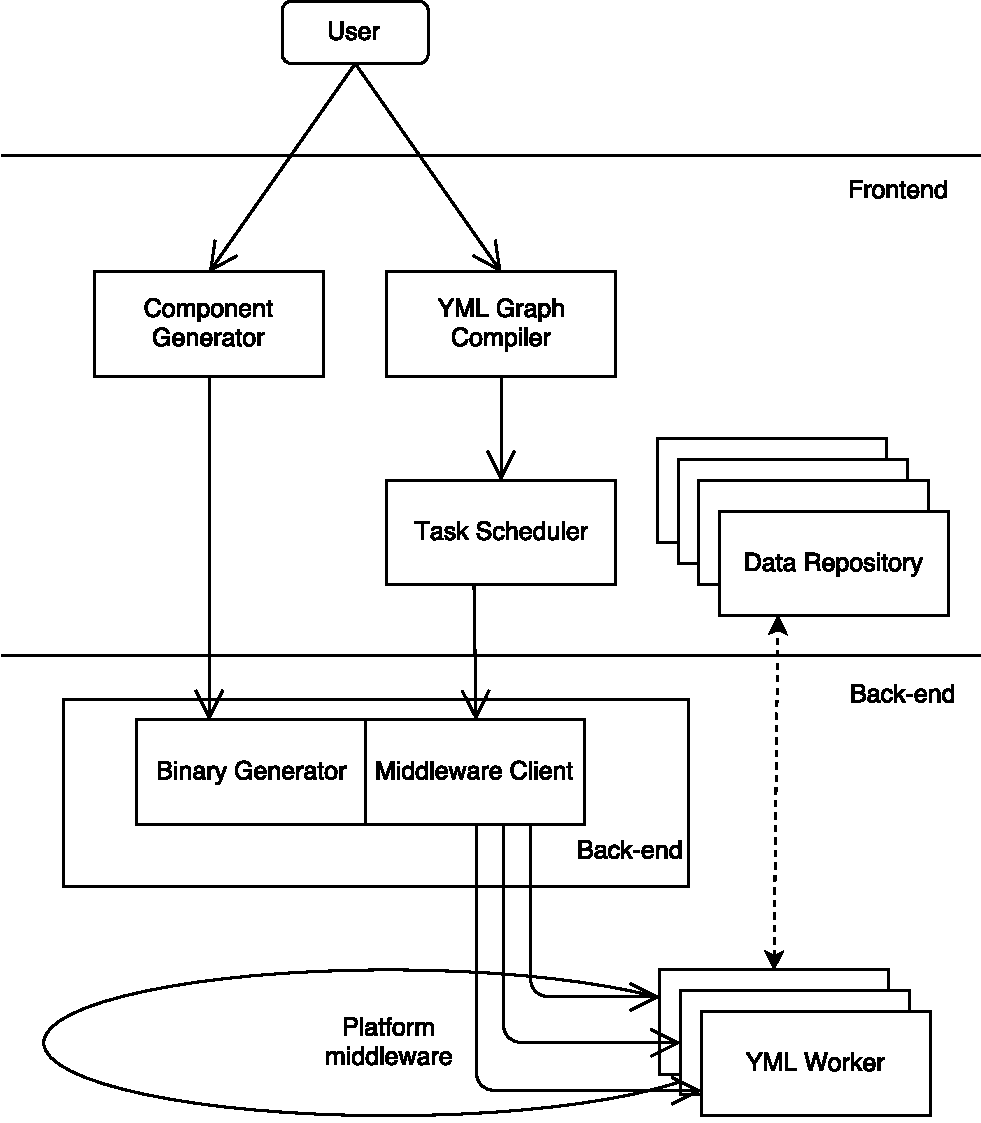
\includegraphics[width=.5\textwidth]{schema.pdf}
\end{figure}

\textbf{The component model} defines three classes of components : Graph, Abstract and Implementation.
They are encapsulated using XML.
They are made to hide the communication aspect and the code related to data serialization and transmission.

\begin{itemize}
	\item Graph components contain the name, a description of the application and the graph written using YvetteML.
	This component also defines global parameters.
	They are data that can be used in components.
	Abstract components are called with the keyword \textit{compute}, their name and the list of parameters they need.
	\item Abstract components contain the name, the type (abstract) and a description of the component.
	They also define the parameters of the data coming from the global application and describe their use in the component (if the data are consumed, modified or created).
	\item Implementation components contain the name, the type (implementation), a description, the name of the abstract component associated, the language used, the external libraries that YML has to deploy and the source code.
	The links of the libraries are installed in YML then they can be used in the implementation component and YML deploys them when needed.
	The source code can also be written in several programming languages, including, for the moment, C/C++, Fortran or XscalableMP (XMP) \cite{XMP}.
\end{itemize}

These categories of component allow re-usability, portability and adaptability.

\textbf{The Component generator} registers the Abstract and Implementation components in YML and the data they need.
The Component generator starts to check if the abstract components exist then it extracts the source code and the information needed to create a standalone application.
The generator also adds the code to import and export the data from the file system.
Afterwards, the Component generator calls the Binary Generator (Figure \ref{fig:schema}) to compile the generated application.
It uses the compiler associated to the language filled in the Implementation component.

\textbf{The Graph compiler} generates the YML application by compiling the Graph component.
It checks that all the components called exist, then verifies that the YvetteML graph is correct.
It also extracts the control graph and the flow graph from the Graph component and the Abstract components.
It creates a binary file containing the application executable with the YML scheduler.

\textbf{The scheduler} manages the computational resources and the data of the application during its execution.
A set of processes is allowed to YML to run the application.
The scheduler explores the graph at runtime (Figure \ref{fig:schema}) to determine which component has to be run.
A component can be run if the execution of the previous components is finished, the data and the computational resources are available.
The scheduler runs the component of the application on a subset of the processes through a worker.
The scheduler sends the component (as shown in the Figure \ref{fig:schema}) to a worker through the middleware.
It executes the component on the subset of processes that manages the worker.
Several workers can run at the same time if there are enough processes available.

Data are stored in a repository created in the current repository at the launch of the application.
The data are read by the components that need them.
The components produce or/and create data and write them in the repository.

\subsubsection{XcalableMP}
XcalableMP (XMP) \cite{XMP} is a directive-based language extension for C and Fortran,  which allows users to develop parallel programs for distributed memory systems easily and to tune the performance by having minimal and simple notations.
XMP supports (1) typical parallelization methods based on the data-/task-parallel paradigm under the "global-view" model and (2) the co-array feature imported from Fortran 2008 for "local-view" programming.

The Omni XMP compiler translates an XMP-C or XMP-Fortran source code into a C or Fortran source code with XMP runtime library calls, which uses MPI and other communication libraries as its communication layer.

Figure \ref{fig:xmpprog} is an example of XMP programming.
A dummy array called {\bf template} indicates data index space and is distributed onto the nodes.
Each element of the array is allocated to the node where corresponding template element is distributed.

\begin{figure}
	\centering
	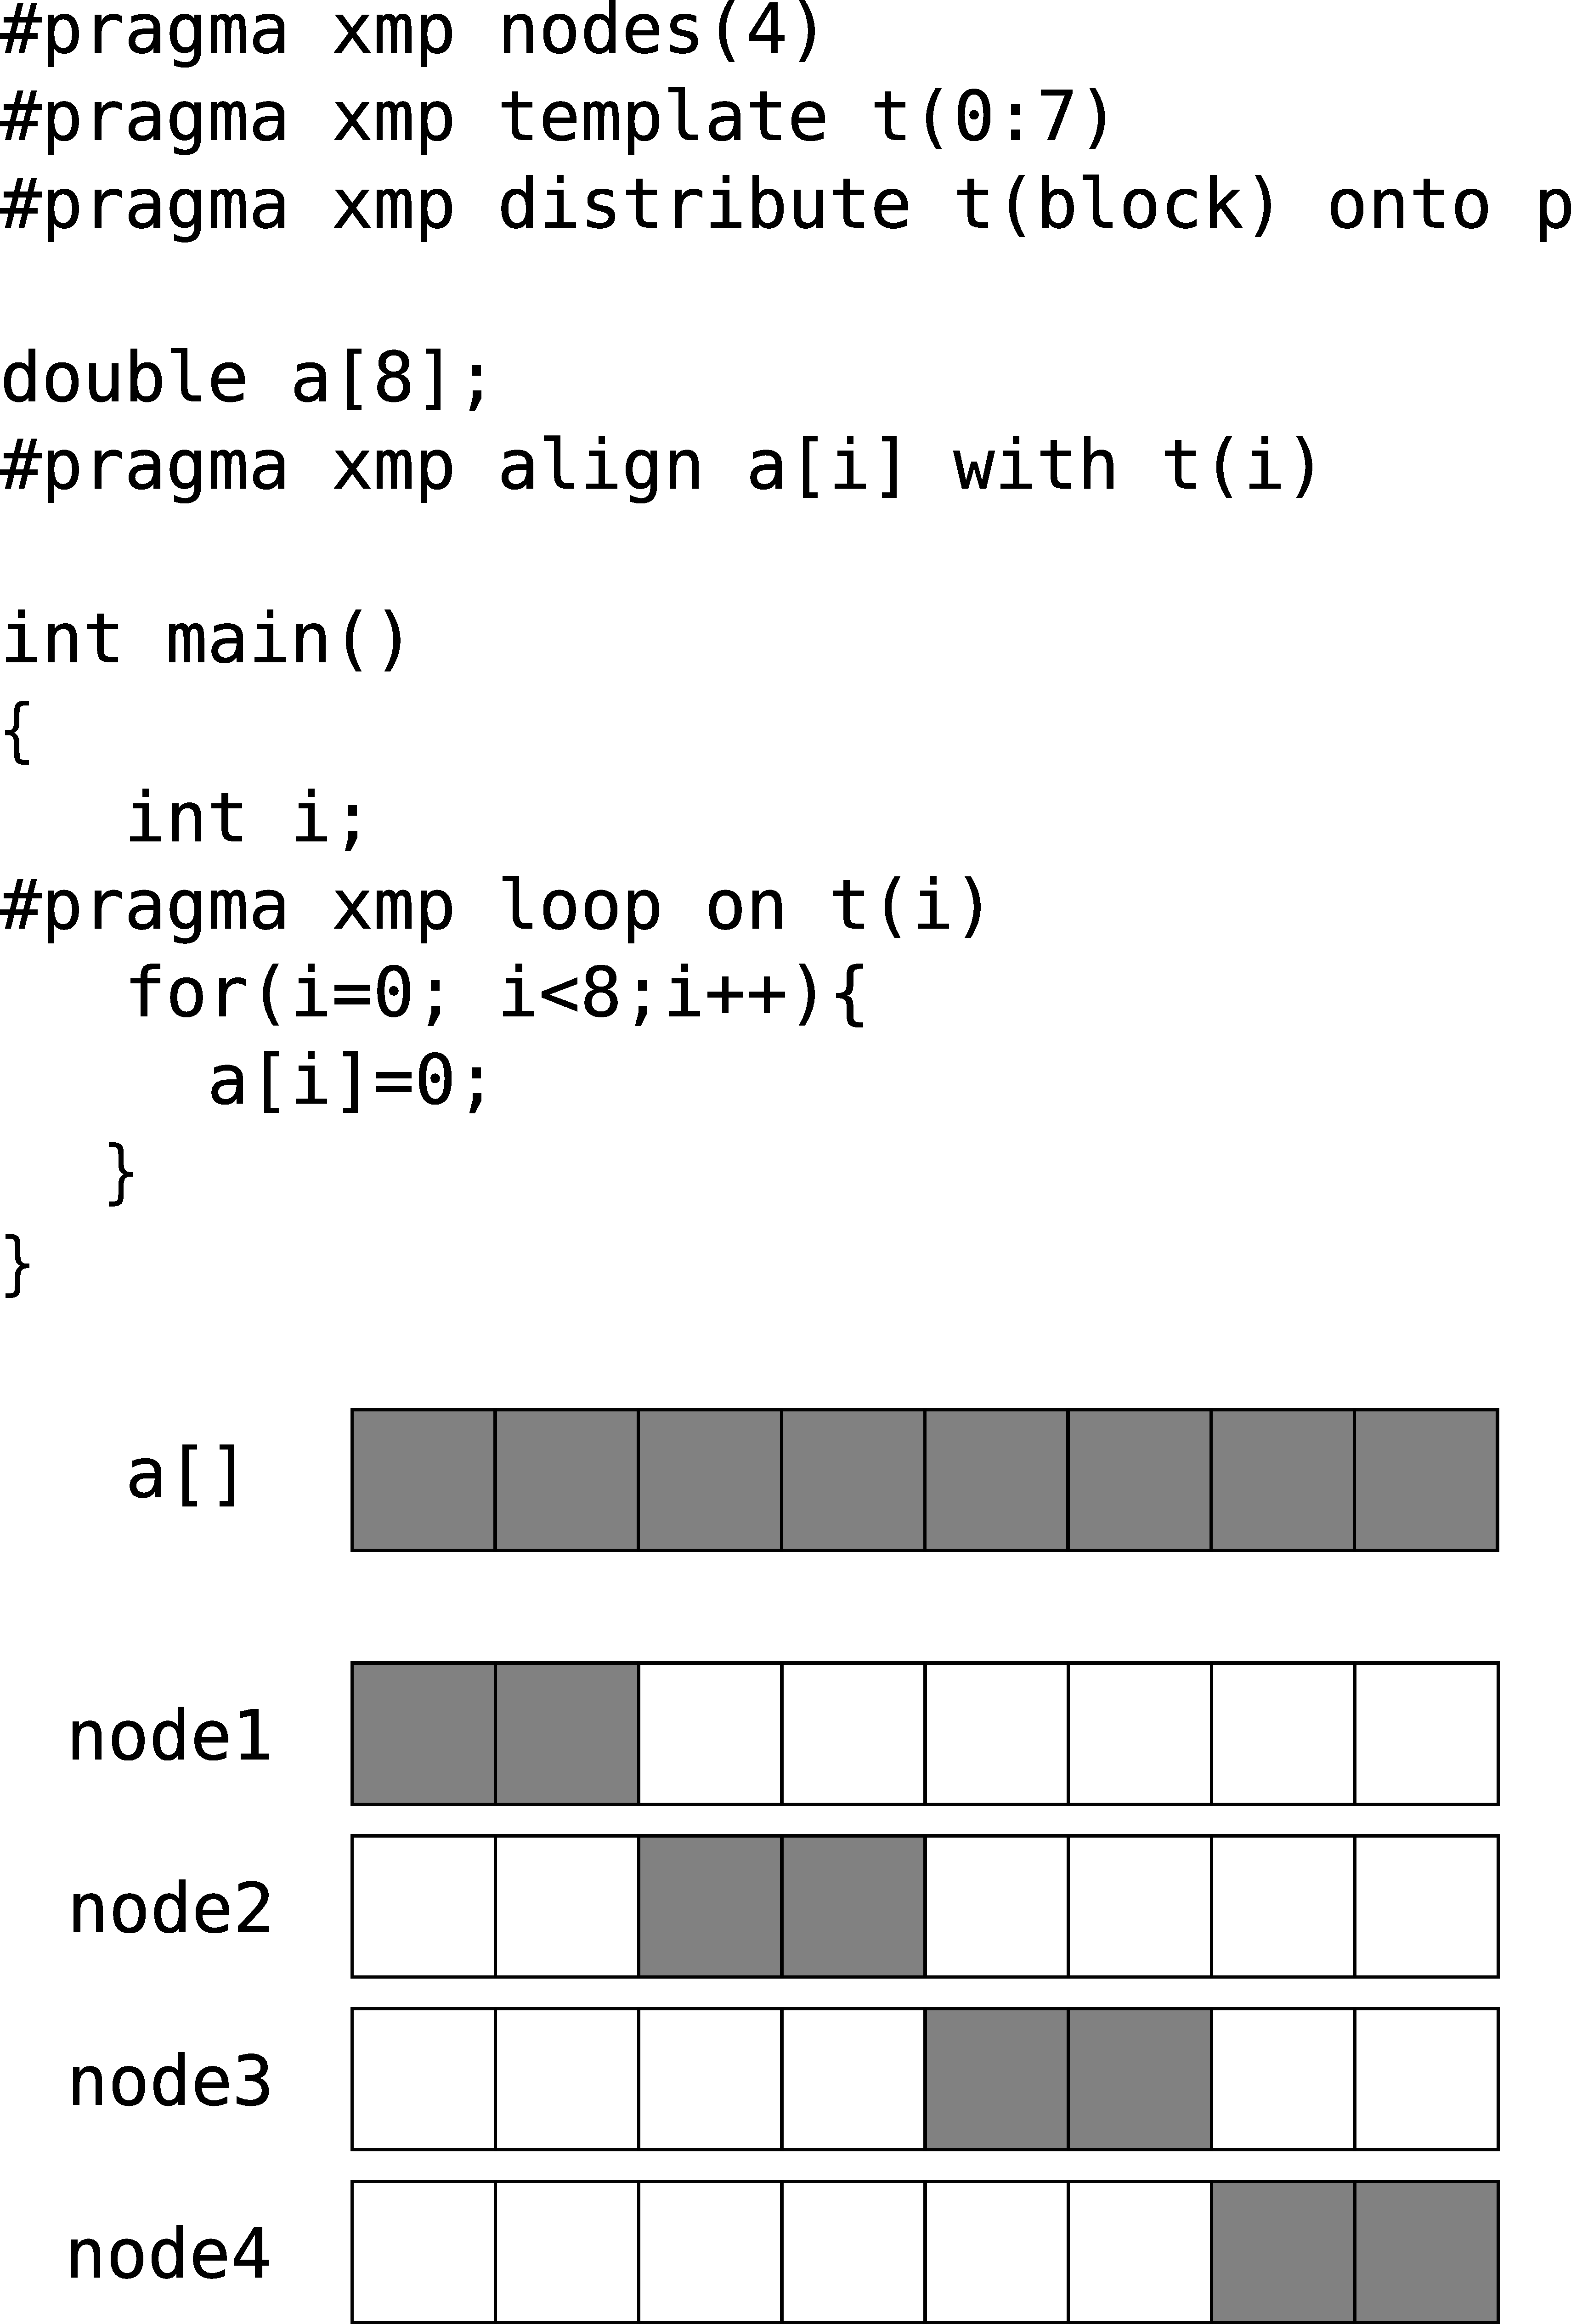
\includegraphics[width=.35\textwidth]{xmp-example.pdf}
	\caption{Example of XMP programming\label{fig:xmpprog}}
\end{figure}

\subsubsection{YML/XMP}
For the experiments, we use XMP to develop the YML components as introduced in \cite{TsSHP2013}.
This allows two levels programming.
The higher level is the graph (YML) and the second level is the PGAS component (XMP).
In the components, YML needs complementary information to manage the computational resources and the data at best : the number of XMP processes for a component and the distribution of the data in the processes (template).
Line 5 to 11 from Listing \ref{lst:yml_task} shows the additional information provided to YML by the user in the implementation component in XMP.
With this information, the scheduler can anticipate the resource allocation and the data movements.
The scheduler creates the processes that the XMP components need to run the component.
Then each process will get the piece of data which will be used in the process from the data repository.

\begin{figure*}[t]
\lstinputlisting[style=customcode,
caption=XMP implementation component for YML\label{lst:yml_task}]{chapters/languages/yml_task.query}
\end{figure*}

In this approach, there are no global communications along all the processors (like scalar products or reductions) in the application since applications are divided on component calls that use a subset of the computational resources allowed to the application.
The components running at the same time don't communicate with each other and are run independently.
Global communications take time and consume a lot of energy so reducing them and finding other ways to get the same results saves time and is more power efficient.

\begin{figure*}
\lstinputlisting[style=customcode,
caption=Abstract component for YML\label{lst:yml_task_abst}]{chapters/languages/yml_task_abst.query}
\end{figure*}

\subsubsection{Task definition}
In YML, implementing a task means to create a component.
There is two type of components to implement; an abstract component and an implementation component which will be be implemented with XMP in this case.
Listing \ref{lst:yml_task_abst} shows an example of abstract component.
Line 2 gives the type of component (abstract), the name of the component and a brief description.
This name will be used in the implementation component and to call the task.
Line 4 and 5 define 2 \textit{Matrix} parameters; one is in input and the other one is used in input and output.
The second matrix will be modified by this task.

Listing \ref{lst:yml_task} contains the actual implementation of the component.
Line 2 sets the name of this component and also tells which abstract component it implements.
Line 4 gives the language used to implement this component.
The languages can also be C++ and Fortran as detailed previously.
It uses XMP in this case.
Line 4 also sets how much cores will be used to run the task on.
In this case, we use a 2D array of $32 \times 32$ CPUs.
Line 5 to 11 describe how to distribute the Matrix \textit{A0} and \textit{B0} (defined in the abstract component) on the allocated cores.
It also defines the size of the matrices used ($512 \times 512$).

The code of the task is contained in the \textit{header}, \textit{source} and \textit{footer} tags.
The code inside the \textit{header} tag will be put at the end of the header part of the generated C source file of the component.
The code from \textit{source} tag is put in the main and the code from the \textit{footer} tag will be put at the end of the generated C file.

\subsubsection{Dependency definition}
Dependencies are defined while creating the graph of tasks.
Listing \ref{lst:yml_graph} shows a YML graph with dependencies between the tasks.
Tasks are called with the keyword \textit{compute}, the name of the component provided in the abstract component and the parameters of the task.
They can be called in bulk with loops.
\textit{for} and \textit{par} are the two statements which can be used to repeat statements.
The \textit{for} loop can be used to call task one after the other.
It creates dependencies to wait for the previous task to be finished before launching the next.
The \textit{par} loop launch every task in the loop body at the same time.
A \textit{par} loop is used on lines 10 and 13 in Listing \ref{lst:yml_graph}.
There is also a \textit{par} statement which can be used alongside with \textit{//} to launch several tasks at the same time.

Additional dependencies can be expressed by using YML locking event system.
The \textit{wait} and \textit{notify} keywords are used to manage the events.
\textit{wait} locks the following operations until the event is released by a \textit{notify} on the same event.
For instance, on line 22, the \textit{XMP\_inversion} task depends on the \textit{p[i][i][i]} which is locked by a \textit{wait}.
This event will be released by the \textit{notify} on line 17 when $k = i + 1$ and $j= i + 1$.
It means that the task \textit{compute XMP\_inversion(A[i][i],B[i])} depends on the task \textit{compute XMP\_prodDiff(A[k][i],A[i][j],A[k][j])}.
This event system is used to infer a graph of dependencies.
It is used to schedule the tasks.

\begin{figure*}
\lstinputlisting[style=customcode,
caption=YML Graph\label{lst:yml_graph}]{chapters/languages/yml_graph.query}
\end{figure*}

\subsubsection{Data definition}
In YML, data types have to be registered so that it is able to manage them.
They are stored in the \textit{DefaultExecutionCatalog/generators} directory in YML configuration files.
Listing \ref{lst:yml_data} shows an example of the functions to implement with the \textit{Matrix} used in the abstract component.
There is three functions to implement.
The first is \textit{$<$type\_name$>$\_MPI\_Type} which return the \textit{\_MPI\_Datatype} used to import and export the data associated to the type in a task.
It can be a custom MPI type.
\textit{$<$type\_name$>$\_import} and \textit{$<$type\_name$>$\_export} are the two other functions to implement.
They are used to import and export the type from the file system.
MPIIO is used to do so in the Matrix type.

\begin{figure*}
\lstinputlisting[style=customcode,
caption=Matrix XMP type\label{lst:yml_data}]{chapters/languages/yml_Matrix.xmptype.h}
\end{figure*}

\subsubsection{Graph execution}
The graph is executed by launching the \textit{.yapp} application with the \textit{yml\_scheduler}.
This application is produced by \textit{yml\_compiler}.
With XMP back-end, \textit{yml\_scheduler} is launched with \textit{mpirun -n 1 yml\_scheduler my\_app.yapp}.
It will enable YML to launch tasks in the distributed environment.

\subsubsection{Granularity}
With the XMP back-end, tasks are MPI based applications implemented with XMP so they use multi-processes technology.
Each XMP task can run on several nodes of the global number of nodes associated to the application.
These tasks are coarse-grain.

The C back-end provides multi-threaded tasks.
These tasks can be run on one node.

\subsubsection{Tasks re-usability}
Implementation and abstract components can be reused in another application by calling them again with the \textit{compute} keyword.
However, components implemented in XMP have their number of cores used and size of data fixed.
Unfortunately, they cannot be changed dynamically.
It means that the components have to be recompiled each time one of those parameters is changed or that multiple versions if the component with different parameters have to coexist.

\subsubsection{Scheduling}
When a task dependencies are satisfied, the task is put in the execution queue.
The tasks in this queue are executed when the resources are available.
Furthermore, the tasks are launched on the resources they ask in their implementation.

\subsubsection{Type of graph}
The user defines the control flow graph while giving the dependencies between the tasks.
However, the data flow graph can be extracted from the control flow graph and the access mode of the data provided in the abstract component.

\subsubsection{GPU support}
No support for GPUs has been directly implemented in YML.




\subsection{Pegasus}
Pegasus \cite{DSSBG2005} \cite{DVJRC2015} is a Workflow Management System.
It allows the user to express multi-step computational tasks through a directed acyclic graph (DAG), where the nodes are tasks and the edges denote the task dependencies.
The tasks can be everything  from short serial tasks to very large parallel tasks (MPI for example) surrounded by a large number of small, serial tasks used for pre- and post-processing.

Pegasus provides helpers to execute workflow-based applications in different environments like desktops, clusters, grids and clouds.
It automatically maps high-level workflow descriptions onto distributed resources.
It also locates the necessary input data and computational resources needed during the workflow execution.
Pegasus enables scientists to construct workflows in abstract terms.
It can be linked with several middlewares (HTCondor DAGMan \cite{ThaTL2002}, Globus, or Amazon EC2).

Pegasus is fault tolerant.
Indeed, when there is errors, it can retry the tasks, retry the entire workflow, checkpoint its execution, re-map part of the workflow, try alternative data sources and as last resort, provide a list of the remaining tasks.
Storage is cleaned up during the execution of the workflow.
Thus, data-intensive workflows can get enough space to run their tasks on resources with low-capability storage.
Pegasus also keeps track of what has been done, where, which software was used and their parameters.

Pegasus has been used in a number of scientific domains including astronomy, bioinformatics \cite{PRBBF2016}, earthquake science , gravitational wave physics, ocean science, and others.

\subsubsection{Task definition}
In Pegasus, tasks are called \textit{Job}.
Listing \ref{lst:pegasus_task} shows how to define and register a \textit{Job} into Pegasus.
DAX Python API is used to generate the XML file that will be treated by Pegasus to launch the jobs on the available resources.
Line 1 defines the graph which will be populated with the jobs.
Then, line 3 to 7 define the Job with its name space, name and version.
The name of the job corresponds to the name of the Executable defined and registered in Listing \ref{lst:pegasus_reg_exe}.
An executable is registered into a graph with the \textit{addExecutable} method.

\begin{figure*}[h]
\lstinputlisting[style=customcode,
caption=Pegasus task\label{lst:pegasus_task}]{chapters/languages/pegasus_task.py}
\end{figure*}

A job can also pass arguments to the executable with the \textit{addArgument} method.
String and files can be passed as arguments.
A file \textit{c1} is created and will be used as output as stated on line 7.
An already existent file \textit{b1} will be used as input.
The files have registered into the job with the \textit{uses} method so that Pegasus runtime will be able to manage is and move it across the network if needed.
Finally, the job is registered into Pegasus graph by using the \textit{addJob} method from the graph (on line 8 from \ref{lst:pegasus_task}).

A file could be used as input and output however, the \textit{Link.INOUT} property cannot be used.
It does not seem to be implemented.
Therefore, a task cannot modify a file and needs to have an output distinct from the input.
Moreover, each file is considered as an output by default.
They will be transfered back to the user by the runtime, even the temporary files that has to be created due to the impossibility to use a file name as input and output.
The user has to manually set the temporary files as not wanted as output instead of modifying a file.
This decreases the complexity of the runtime since the data files will be unique.

\begin{figure*}[h]
\lstinputlisting[style=customcode,
caption=Register executable in Pegasus\label{lst:pegasus_reg_exe}]{chapters/languages/pegasus_register_exe.py}
\end{figure*}

\subsubsection{Dependency definition}
Dependencies are simple to add into a Pagasus graph with the Python interface.
Indeed, the graph has a method called \textit{addDependency} that takes the dependency as parameter.
A dependency can be declared by providing if the parent and child jobs.
Listing \ref{lst:pegasus_dep} shows an example of such a dependency.

\begin{figure*}[h]
\lstinputlisting[style=customcode,
caption=Dependecy in Pegasus\label{lst:pegasus_dep}]{chapters/languages/pegasus_dep.py}
\end{figure*}

\subsubsection{Data definition}

Pegasus jobs call executables that process files so the user has to use data files that match the format used by the executables to read or write data from file.
The user has to register data files either as intermediary to transfer data from a job to another as described above or registered to the graph which will be used as input and/or output of the jobs performed by the application.
Listing \ref{lst:pegasus_file} shows an example of files registered to the graph.

\begin{figure*}[h]
\lstinputlisting[style=customcode,
caption=File registration in Pegasus\label{lst:pegasus_file}]{chapters/languages/pegasus_file.py}
\end{figure*}

\subsubsection{Graph execution}
Pegasus Python API generates a DAX which can be executed by Pegasus \textit{pegasus-plan} command.
It will submit the jobs to the resources available to the application and manage the input and output data files.

\subsubsection{Granularity}
The jobs can be anything between short one threaded application to large scale multi-node applications based on MPI.

\subsubsection{Tasks re-usability}
Jobs can be reused in another application if they use the same arguments and files as input otherwise, they will have to be rewritten.


\subsubsection{Scheduling}
By default, Pegasus uses HTCondor DAGMan \cite{ThaTL2002} as underline work-flow manager.
Therefore, it uses HTCondor Schedd to schedule the jobs submitted to HTCondor DAGMan.

Pegasus can use  other back-ends as engine.
The scheduling policy will depend on how the engine manage the jobs submitted to it.


\subsubsection{Type of graph}
The user only defines dependencies between Jobs so the graph is a control flow graph.

\subsubsection{GPU support}
Pegasus does not seem to support GPU by itself.
The user should be able to tell Pegasus which tasks need GPU to run on and which resources have GPU available.
Pegasus tasks are implemented on top of an existing executable so this executable has to be able to manage GPUs to run applications on them.



\subsection{Swift}
\subsubsection{Swift}
Swift \cite{ZHCFL2007} \cite{WHWCK2011} is a scripting language for executing many instances of ordinary application programs on distributed and parallel resources.
Swift runs applications as soon as their inputs are available.
The programming is simpler since the user doesn't have to manage the dependencies.
The variables can be assigned only once.
This allows Swift to easily know when to launch a function.
Figure \ref{fig:swift_excode} is an example\footnote{\url{http://swift-lang.org/Swift-T/index.php}} of code which can be translated to the graph of the Figure \ref{fig:swift_exgraph}.
If the variable has been set then the function can use the data.
Otherwise, Swift wait for the variable to be set before launching functions that need this variable.
It simplifies the expression of the parallelism for the system.
Thus, all code will be executed in parallel unless there is a variable unset in a function call.
The function using the unset variable will wait for the variable to be set by another call.
Therefore, there will be sequencing between the two calls.
Swift expressions are evaluated in dataflow order to run the workflows with the most concurrency possible.
It only depends on the data dependencies and the available resources.
Moreover, Swift allow to wrap applications into functions to create more complex scripts.
The functions take files as input and produce files as output.

\begin{figure}[H]
\begin{multicols}{2}
	\begin{lstlisting}[basicstyle=\ttfamily, tabsize=3, frame=single]
	int X = 100, Y = 100;
	int A[][];
	int B[];
	foreach x in [0:X-1] {
		foreach y in [0:Y-1] {
			if (check(x, y)) {
				A[x][y] = g(f(x), f(y));
			} else {
				A[x][y] = 0;
			}
		}
		B[x] = sum(A[x]);
	}
	\end{lstlisting}
	\caption{Example of Swift code \label{fig:swift_excode}}
	\centering
	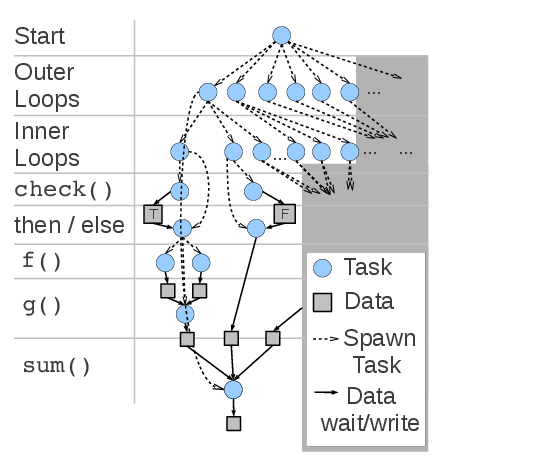
\includegraphics[width=.45\textwidth]{swift_spawngraph}
	\caption{Graph translation of the code\label{fig:swift_exgraph}}
\end{multicols}
\end{figure}

Swift is suitable for Grid.

We found several applications which use Swift.
For instance, \cite{APWXF2011} uses Swift for proteins modelling or \cite{WoiDS2011} for parallel climate data analysis.

\subsubsection{Swift/T}
Swift/T \cite{WAWKL2013} is a new implementation of Swift dedicated to HPC.
It translates the Swift script into a MPI program using Turbine \cite{WAMLK2012} and ADLB (Asynchronous Dynamic Load Balancer) \cite{LusPB2010} libraries.
Turbine is a Tcl library that assemble MPI, ADLB and the Turbine dataflow library.
ADLB is a software library designed to build scalable parallel programs.

Swift/T has two main level of programming : the Swift script and the Leaf functions.
The Swift parallel script correspond to the high grain graph and the leaf functions to the tasks.
The heavy computations are located in the leaf functions.
Since Swit/T uses Swift scripts, the variable assignments and the expression of the parallelism works the same way.

There is three types of leaf functions in Swift/T :
\begin{enumerate}
	\item Extension functions : Tcl (language used in Turbine) or native code functions like C, C++, Fortran or MPI (possibility to call them as parallel functions).
	These functions primarily operate on in-memory data, and are appropriate for high-performance computing.
	\begin{lstlisting}[basicstyle=\ttfamily, tabsize=3, frame=single, language=C, caption=C function\label{lst:swift_cfunc}]
	#include <stdio.h>
	#include <stdlib.h>

	double* b(double* v, int length) {
	  int i;
	  double sum = 0.0;
	  printf("length: %i\n", length);
	  for (i = 0; i < length; i++) {
	    sum += v[i];
	  }
	  printf("sum: %f\n", sum);
	  double* result = malloc(sizeof(double));
	  result[0] = sum;
	  return result;
	}
	\end{lstlisting}
	Listing \ref{lst:swift_cfunc} is the code of the \textit{b} function used in the example\footnote{\url{http://swift-lang.github.io/swift-t/leaf.html\#_complete_example_2_simple_c_function}} of a C leaf function.

	\begin{lstlisting}[basicstyle=\ttfamily, tabsize=3, frame=single, caption=Creation of the Tcl package\label{lst:swift_ctclpackage}]
	rm *.o
	swig -module b b.i
	gcc -c -fPIC b.c
	gcc -c -fPIC $TCL_INCLUDE_SPEC b_wrap.c
	gcc -shared -o libb.so b_wrap.o b.o
	tclsh make-package.tcl > pkgIndex.tcl
	\end{lstlisting}
	Listing \ref{lst:swift_ctclpackage} shows how to create the wrapper of the C function which will be called in the Tcl function.

	\begin{lstlisting}[basicstyle=\ttfamily, tabsize=3, frame=single, caption=Tcl wrapper around the C funtion\label{lst:swift_ctclfunc}]
	namespace eval b {
	    # v is formatted as a Turbine blob a list of [ pointer length ]
	    # The pointer is a simple Tcl integer
	    # The length is the byte length
	    proc b_tcl { v } {

	        # Unpack the list
	        set ptr [ lindex $v 0 ]
	        set len [ lindex $v 1 ]

	        # Get the number of numbers to sum
	        set count [ expr $len / [ blobutils_sizeof_float ] ]

	        # Convert the pointer number to a SWIG pointer
	        set ptr [ blobutils_cast_int_to_dbl_ptr $ptr ]

	        # Call the C function
	        set s [ b $ptr $count ]

	        # Pack result as a Turbine blob and return it
	        set r [ blobutils_cast_to_int $s ]
	        return [ list $r 8 ]
	    }
	}
	\end{lstlisting}
	Listing \ref{lst:swift_ctclfunc} shows how to use the C function inside a Tcl function.
	This Tcl function is used in the Swift application.
	Listing \ref{lst:swift_cswiftapp} shows how to call a Tcl function from a Swift application.

	\begin{lstlisting}[basicstyle=\ttfamily, tabsize=3, frame=single, caption=Call of the Tcl wrapper by a Swift application\label{lst:swift_cswiftapp}]
	import blob;
	import io;

	(blob sum) b(blob v) "b" "0.0"
	[ "set <<sum>> [ b::b_tcl <<v>> ]" ];

	file data = input_file("input.data");
	blob v = blob_read(data);
	blob s = b(v);
	float sum[] = floats_from_blob(s);
	printf("sum (swift): %f", sum[0]);
	\end{lstlisting}
	\item app functions: Functions that call to a command-line program (the shell).
	These functions primarily operate on files, and are appropriate for ordinary workflows.
	\item External scripting functions: Functions that call into an in-memory interpreter in another scripting language, such as Python (Listing \ref{lst:swift_pythonswift}), R (Listing \ref{lst:swift_Rswift}), or \textbf{Julia} (Listing \ref{lst:swift_juliaswift}).
	\begin{lstlisting}[basicstyle=\ttfamily, tabsize=3, frame=single, caption=Call of python code by a Swift application\label{lst:swift_pythonswift}]
	import io;
	import python;
	import string;

	global const string numpy = "from numpy import *\n\n";

	typedef matrix string;

	(matrix A) eye(int n)
	{
	  string command = sprintf("repr(eye(%i))", n);
	  matrix t = python_persist(numpy, command);
	  A = replace_all(t, "\n", "", 0);
	}

	(matrix R) add(matrix A1, matrix A2)
	{
	  string command = sprintf("repr(%s+%s)", A1, A2);
	  matrix t = python_persist(numpy, command);
	  R = replace_all(t, "\n", "", 0);
	}

	matrix A1 = eye(3);
	matrix A2 = eye(3);
	matrix sum = add(A1, A2);
	printf("2*eye(3)=%s", sum);
	\end{lstlisting}


	\begin{lstlisting}[basicstyle=\ttfamily, tabsize=3, frame=single, caption=Call of R code by a Swift application\label{lst:swift_Rswift}]
	import io;
	import string;
	import R;

	global const string template =
	"""
	  x <- %i
	  a <- x+100
	  cat("the answer is: ", a, "\\n")
	""";

	code = sprintf(template, 4);
	s = R(code, "toString(a)");
	printf("the answer was: %s", s);
	\end{lstlisting}


	\begin{lstlisting}[basicstyle=\ttfamily, tabsize=3, frame=single, caption=Call of  Julia code by a Swift application\label{lst:swift_juliaswift}]
	import io;
	import julia;
	import string;
	import sys;

	start = clock();
	f =
	"""
	begin
	 f(x) = begin
	          sleep(1)
	          x+1
	        end
	 f(%s)
	end
	""";
	s1 = julia(sprintf(f, 1));
	s2 = julia(sprintf(f, 2));
	s3 = julia(sprintf(f, 3));
	printf("julia results: %s %s %s", s1, s2, s3);
	wait (s1, s2, s3) {
	  printf("duration: %0.2f", clock()-start);
	}
	\end{lstlisting}
\end{enumerate}

\section{Analysis and First Evaluation of the Languages}

HPX is a task based programming model.
The tasks are run as lightweight processes on the resources managed by HPX runtime.
The data and the tasks can be transfered across distributed nodes.
It uses modern C++ which starts to be used more often in HPC applications.
It extends C++ future-based (tasks) multi-threaded programming to distributed.
Moreover, HPX is very close to C++ standards so it provides an interface which is supported and documented.
Those are the points for which we are choosing HPX.

PaRSEC is a runtime which manages data and launches tasks.
It also provides several DSLs to define and implement tasks.
Two DSLs are already available.
They allow the user to describe the dependencies between the tasks and how the tasks are implemented.
PaRSEC has good performances compared to the one obtained with HPX as shown in \cite{GurhP2020} .

YML+XMP is a distributed and parallel task based programming model where each task is also distributed and parallel.
This programming has been selected because it has two level of programming, the graph which is the high level and the parallel and distributed task which is the second level.
\cite{GurhP2020} shows that YML+XMP has a better scalability compared to the other programming models.
However, the performances of YML+XMP are its weak points due the use of the file system to perform the communications.
YML+XMP is not the only programming model to use is to make the communications.
Indeed, Pegasus also use files to transfer data from a task to the others.

Legion will not be used due to its way of defining tasks via a tree of tasks which is less natural than a graph of tasks.
Moreover, Legion verbose API is difficult to use.
Finally, Legion performances with the default data mapper are not as good as the performances obtained with the other languages as shown in \cite{GurhP2020} while using Regent to generate Legion code.
Therefore, Regent will not be used too.


TensorFlow is focused in Machine Learning and Neural Networks.
It is well adapted to train models and to process data with those models.
It offers a high level API to easily create and train models.
In TensorFlow, the Operation is the main way to apply computations on data stored into Tensors aside the Machine Learning API.
However, Operations can only be implemented by adding it directly into TensorFlow code and by recompiling it.
Therefore, it is not well adapted to other kind of applications and will not be used to implement the Kirchhoff Migration.
%TODO not used for which application ?

CnC does not seem to be used a lot and does not seem maintained anymore.
Thus, CnC will not be used to implement applications.

OmpSs uses the same kind of approach as OpenMP.
It uses directives to parallelize sections of code.
However, the execution model is different but it still produces multi-threaded applications whereas distributed programming models are considered in this study.

Swift is a parallel programming model where the tasks are also parallel and distributed.
However, the data are sent to the tasks as blobs, an array of bytes, which is copied in each process of the tasks.
Therefore, the distribution of the data is not optimal since each process of the task has a copy of the whole data instead of a part of it.
Furthermore, the user has to write interface with the libraries that will be used as tasks.
This interface consists of several Tcl wrappers and automatic interface generation.
This process could be could be fully hidden from the user.
Swift will not be studied further fo those reasons.

\section{Application Deployment with Containers}
